% !Mode:: "TeX:UTF-8"
\chapter{西青大学城运用GASA-Hopfield 算法求解运输问题}
\section{集成的必要性与可行性}
我们前面介绍到Hopfield神经网络可以很好的解决TSP问题,但是他在解决优化问题时存在着容易求解得到非法解,或者容易收敛到局部最优解,前者随着TSP问题城市数量的增多,非法解出现的频率会逐渐增大。后者会导致最优解的质量得不到保证。本项目在算法上属于王银年在2009年提出的3PM交叉算子的模拟退火算法,但由于求解时间较长,收敛较慢,所以对算法的选择操作进行了重写,并且改变了算法参数,与结束条件。
\section{集成的方法}
\label{jcff}%集成方法
\subsection{单源最短路}
在本例中由于每个地点之间并不直接通达,而是中间经过其他地点后相通,所以为了求解任意两个城市之间的路径我们采用了单源最短路算法-Dijkstra算法:
\par
该算法设置一个集合P,来记录在其求解的图中的最短路顶点,在算法开始时,会将原点放入该集合中,然后算法依次遍历并且将新遍历的点并入集合中,然后更新最短路径,与其路径权值。在算法运行过程中会创建两个中间变量,$dist[]$数组与$path[]$数组。其中$dist$数组记录原点到图中各个顶点的路径长度,$path$表示从原点到某一顶点最短路径的前驱节点的索引值。算法结束后也以此变量来反推最短路径。下面算法中V表示图中的点集,下面给出其算法步骤:
\par
$Step \quad 1: \quad $数据初始化,P集合将原点包含进去,$dist[i] = distance[0][i],\quad i = \{1,2,3,\cdots n-1\}$
\par
$Step \quad 2: \quad $在$V-P$中找到某点$v_k$,该点满足$dist[j] = Min\{dist[i] | v_i \in V-P\}$,令$S = S \cup {k}$。
\par
$Step \quad 3: \quad $求改从$v_0$出发到集合$V-P$中任意一点$v_k$的距离,其更新公式为:\\
\begin{equation}
    \begin{aligned}
        if \quad dist[j]+ distance[j][k] < dist[k] :\\
        dist[k] = dist[j]+distance[j][k]
    \end{aligned}
\end{equation}
\par
$Step \quad 4: \quad $重复$Step \quad 2 \sim Step \quad 3$直到图中所有顶点都被包含到了$P$集合中。
\subsection{主程序}
本例的算法属于王银年在2009年提出的3PM交叉算子的模拟退火算法的变种,称为基于遗传模拟退火策略的Hopfield神经网络的优化算法,对适应度函数,遗传子程序到Hopfield程序的过渡部分,交叉,变异方式进行了添加与改动。由于本算法结合了多种算法所以为了方便叙述,我们将本算法简称为GASA-Hopfield算法,下面给出算法的设计步骤:
\par
$Step \quad 1: \quad $输入初始数据,如邻接矩阵,路径矩阵,数据初始化,如种群,网络参数,迭代步长,交叉,变异概率,初始温度,降温幅度,种植温度,退火迭代链长。
\par
$Step \quad 2: \quad $进入遗传算法子程序,见(\ref{ga-zcx}),传入种群,邻接矩阵,网络参数,编译交叉概率。
\par
$Step \quad 3: \quad $将子程序搜索到的最优路径翻译为置换矩阵,并作为Hopfield网络的输入。
\par
$Step \quad 4: \quad $对神经网络输入$U_{xi}(t)$进行初始化;即$U_{xi}(t) = U^{'}_0+\delta_{xi}$,其中$U^{'}_0 = \frac{1}{2}U_0ln(N-1)$,$\delta$为(-1,+1)区间的随机数。
\par
$Step \quad 5: \quad $动态方程计算$\frac{dU_{xi}}{dt}$;
\par
$Step \quad 6: \quad $根据一阶欧拉法对$U_{xi}进行迭代$即:
\begin{align}
    U_{xi}(t+1) = U_{xi}(t) + \frac{dU_{xi}(t)}{dt}\Delta T
\end{align}
\par
$Step \quad 7: \quad $使用sigmoid函数计算$V_{xi}(t)$即:
\begin{align}
    V_{xi}(t) = \frac{1}{2} (1+tanh(\frac{U_{xi}(t)}{U_0}))
\end{align}
\par
$Step \quad 8: \quad $计算能量函数E;
\par
$Step \quad 9: \quad $检查路径合法性,判断是否达到规定迭代次数,若没达到返回$Step \quad 5$。
\par
$Step \quad 10: \quad $输出每次迭代的能量函数,最优路径。以及最终的路径图,最短路程。
\subsection{遗传算法子程序}
\label{ga-zcx}%GA子程序
\par
$Step \quad 1: \quad $对每个种群求解其对应的适应度。
\par
$Step \quad 2: \quad $对种群进行选择,交叉,变异操作。
\par
$Step \quad 3: \quad $对种族的每个染色体执行模拟退火算法子程序,见(\ref{sa-zcx}),传入一个染色体,此温度下链长,邻接矩阵,初始温度,与网络参数。
\par
$Step \quad 4: \quad $对模拟退火得到的优解保留到下一代中,即继续执行选择操作。
\par
$Step \quad 5: \quad $对此次迭代中得到的新解进行适应度计算。
\par
$Step \quad 6: \quad $判断当前温度是否达到终止条件,如果达到则退出子程序,否则对温度进行更新,转$Step \quad 3$,更新算法为:$T_{i+1} = q \times T_i$,其中$q$代表降温速率,以此来调节算法迭代次数。
\subsection{模拟退火算法子程序}
\label{sa-zcx}%SA子程序
\par
$Step \quad 1: \quad $初始化各个变量,将每次迭代的结果存储下来以便筛选最优解。
\par
$Step \quad 2: \quad $对当前解$S_1$使用交换法进行扰动来产生新解$S_2$。
\par
$Step \quad 3: \quad $通过Metropolis准则来判断是否接受新解,即新解优于旧解则接受,若不优于旧解则根据$p = exp(\frac{E(S_{new}-E(x_{old}))}{KT})$概率接受新解。
\par
$Step \quad 4: \quad $在规定的链长下进行迭代,若执行次数达到规定次数则执行退火操作退出子程序。若没有达到规定次数则返回$Step \quad 2$继续执行产生新解并筛选的过程。
\par
以上述算法编写程序,得到以下结果:
\begin{table}[htbp]
    \centering
    \caption{选择操作改进前后运行效率}%选择改前改后
      \begin{tabular}{|l|l|r|r|}
      %\toprule
      \hline 
      情况    & 时间    & \multicolumn{1}{l|}{最优解} & \multicolumn{1}{l|}{平均解} \\
      \hline 
      选择修改前 & 41234s & 0.26  & 0.28 \\
      选择修改后 & 53s   & 0.18121 & 0.218 \\
      %\bottomrule
      \hline 
      \end{tabular}%
    \label{tab:xzgqgh}%
  \end{table}%
\par
根据表(\ref{tab:xzgqgh})后发现,无论是时间上,还是运行结果上都不理想,并且收敛速度较差,在运行时间上,通过分析程序可知,程序的大部分时间用于遗传算法的选择函数上,而收敛速度慢可以看出优质解并不容易遗传到下一代种群中,所以对程序的选择函数进行重写,重写后的选择步骤为:
\par
$Step \quad 1: \quad $对种群中所有个体按照适应度进行排序。
\par
$Step \quad 2: \quad $对该个体进行判断他有$0 \sim n$个个体进入下一代。
\par
$Step \quad 3: \quad $对下一代个体进行填充。
\par
$Step \quad 4: \quad $下一代种群是否填充完毕,如果填充完毕则退出子函数,若没有填充完毕则返回$Step \quad 2$
\par
其中算法中的$n$可以为定值,也可以是种群数与迭代数的一个变量,本论文中取值为定值,由于此选择程序会导致种群过快收敛而导致解空间搜索并不全面,所以本论文将变异概率改为$min\{\frac{iter^s}{(iter + 1)^s}, pm_{max}\}$,其中$s$为定值,$iter$为迭代次数,$pm_{max}$为所允许的变异率最大值。
\subsection{k-means算法}
对于Hopfield网络引入了混合智能算法,虽然提升了算法局部寻优与全局寻优能力,但是解的求解时间也会增加,随着城市数量的增加其求解时间也会出现较长的问题。为了优化算法的求解速率,我们将引入K-means算法来优化求解时间,其算法思想采用了“分而治之”的思想,将大规模TSP问题分解为小规模多个TSP问题,一方面降低了解的规模,减少了求解时间;另一方面避免了大量无效的劣质解的搜索,优化了解的质量。多个小规模TSP问题解决后,采用类间连接将各个类的路径进行相连。下面我们给出K-means算法的流程图:
\begin{figure}[H]
    \centering
    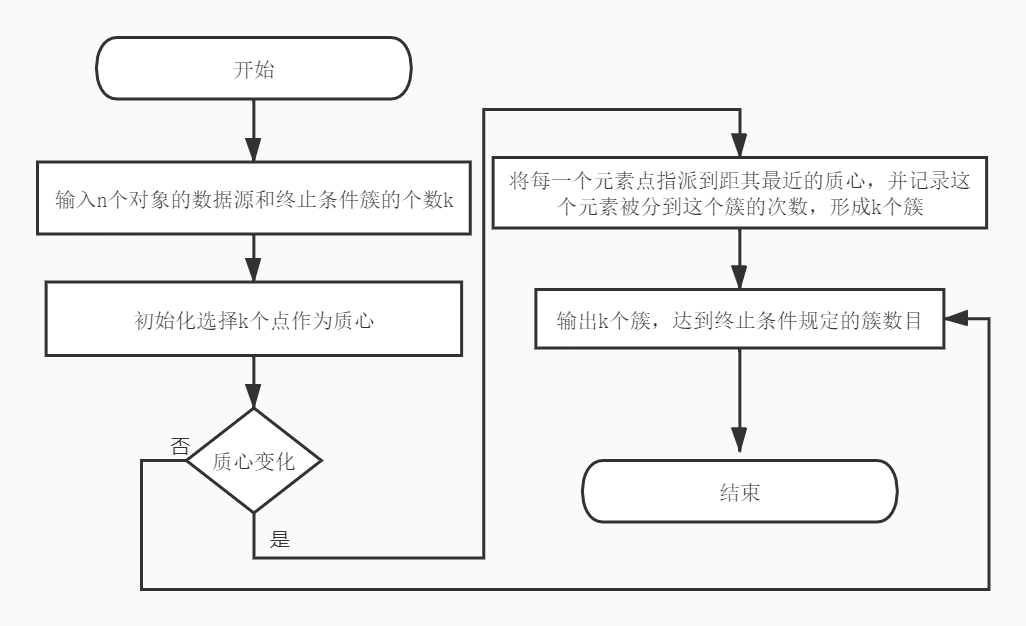
\includegraphics[width=13cm]{figure/kmeans.jpg}%交点实验
    \caption{K-means算法}
    \label{fig:kmeans}
\end{figure}
其中对于最优k值的选取则采用轮廓系数的方法来确定:其轮廓系数的求解方法为:
\begin{align}
    s(i) = \frac{b(i)-a(i)}{max\{a(i), b(i)\}}
\end{align}
其中某一样本$i$到同簇的其余节点的平均距离被称为$a_i$,我们称$a_i$为簇不相似度,即其值越小越属于该簇。一个簇中所有节点的簇不相似度称为该簇的不相似度,也是上式的$a_i$。\\
某一样本$i$到其余某簇的所有样本的平均距离作为该样本与某簇的不相似度,样本$i$到簇$j$的不相似度称为$b_{ij}$,样本$i$的簇间不相似度,定义为:$b_i = min\{b_{i1},b_{i2}, \cdots b_{ik}\}$。其值越小样本越属于该簇。选取好最优分类值后我们开始准备簇间连接。
\par
然后运行主程序对每个类的点进行性求解,然后采用类间连接算法对各个类进行相连,其主要思想为贪心思想,即以第一个簇作为起点簇,依次寻找离此簇最近的点所属于的簇即为簇链的下一个簇元素。
\section{针对运输问题集成Hopfield网络与其他优化算法进行求解}
\subsection{算法实现}
在(\ref{jcff})中我们已经给出了算法流程图,接下来我们偏向于程序实现的角度具体的对改程序的步骤进行阐述。
\begin{figure}[H]
    \centering
    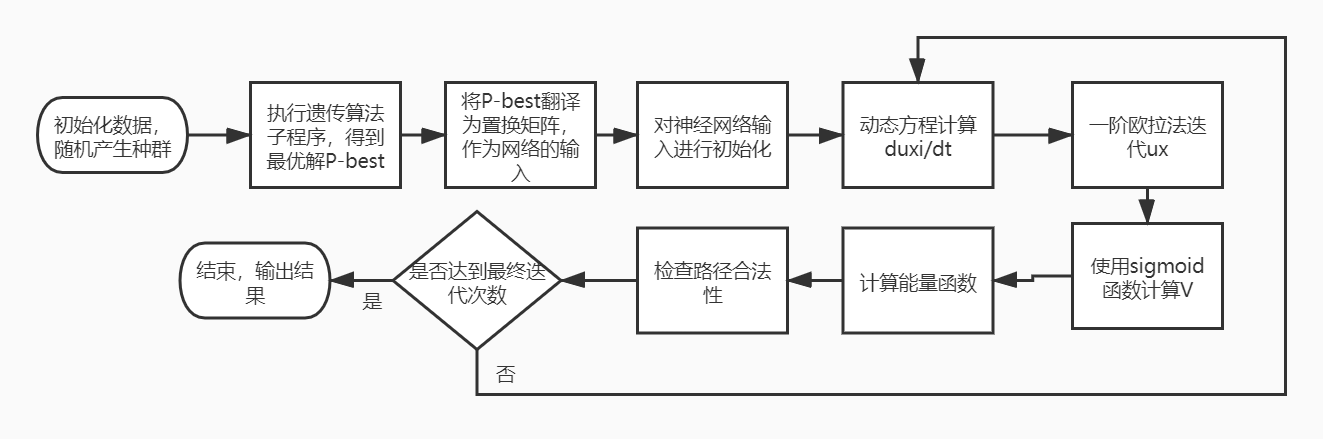
\includegraphics[width=13cm]{figure/main.jpg}%交点实验
    \caption{主程序}
    \label{fig:main}
\end{figure}
上图为主程序的实现,其中需要提前求出的变量为,该区域所有点集的邻接矩阵记为$distance$,进行计算的点集的邻接矩阵$distance_p$,存储所有点集坐标的$x_{pos},y_{pos}$,以及存储第i个点到第j个点的路径的$path-group$,随机生成规定的种群后进入遗传算法子程序,即下图:
\begin{figure}[H]
    \centering
    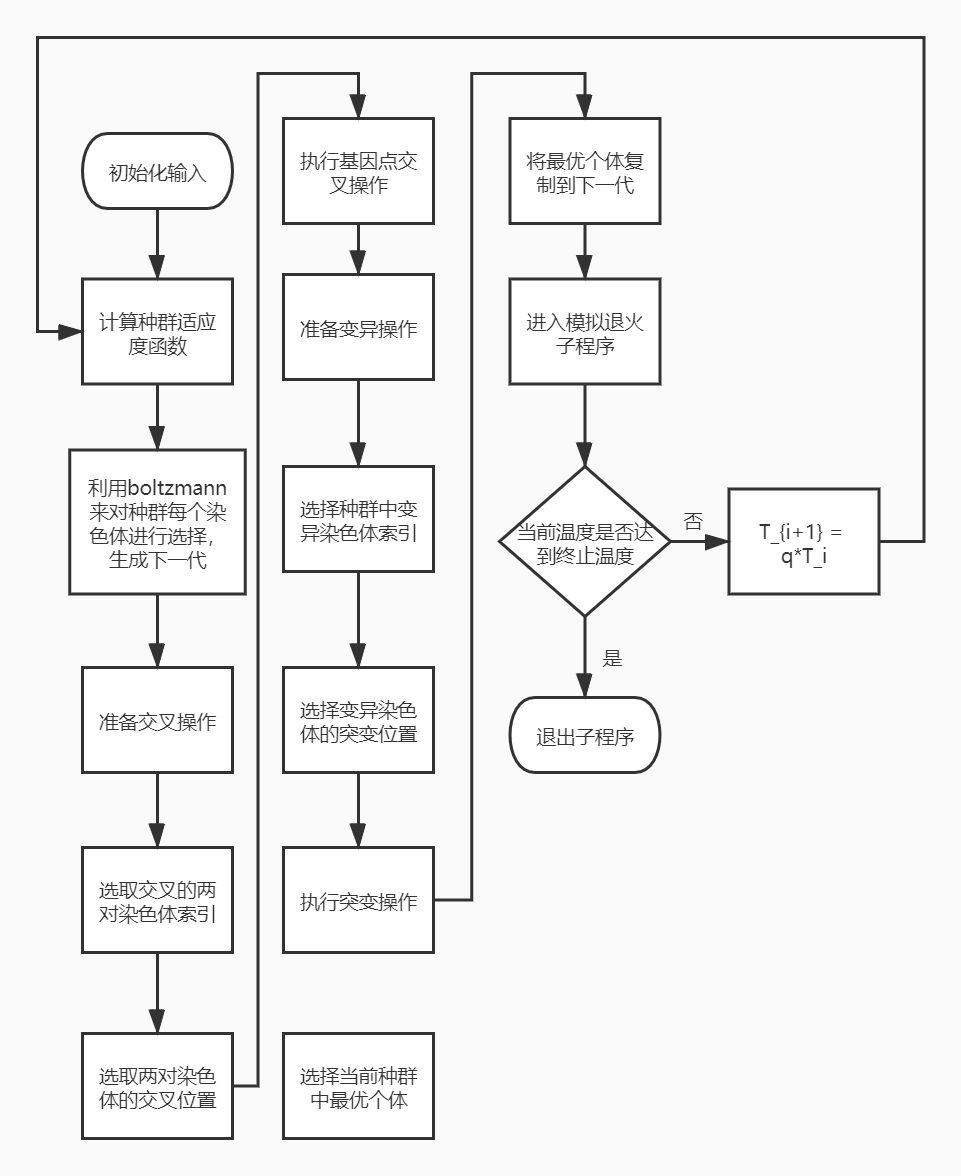
\includegraphics[width=13cm]{figure/main_GA.jpg}
    \caption{遗传算法子程序}
    \label{fig:main_GA}
\end{figure}
在遗传算法子程序中我们的子程序终止条件为温度降为规定温度,并且子程序将种群,$distance_p$,变异率,交换率,网络指标作为初始输入。其中网络指标是由于需要计算能量函数来求解适应度函数。在每次迭代中程序依次执行选择,交叉,变异操作,然后进入模拟退火子程序,对当前代数的最优解附近的空间进行局部搜索,来弥补遗传算法的局部寻优的短板,经模拟退火子程序返回后,在将返回的最优解复制到下一代。然后根据迭代次数的要求判断是否继续迭代。下面我们介绍模拟退火子程序。
\begin{figure}[H]
    \centering
    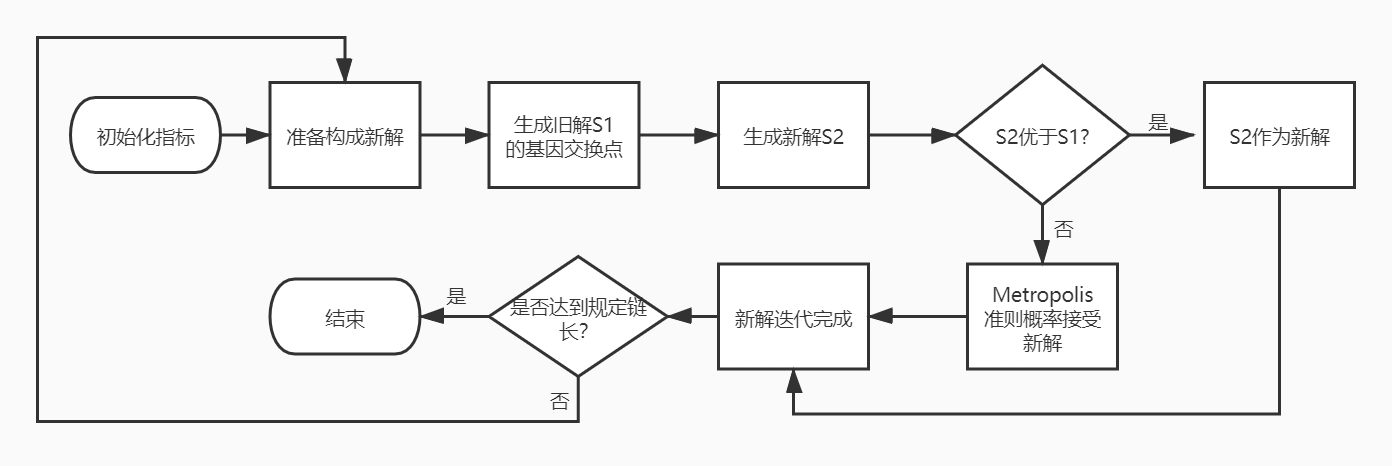
\includegraphics[width=13cm]{figure/main_SA.jpg}
    \caption{模拟退火子程序}
    \label{fig:main_SA}
\end{figure}
模拟退火子程序的设计目的是为了弥补遗传算法局部寻优的不足,并且遗传算法也可以弥补模拟退火算法的全局寻优的短板。模拟退火程序的结束条件生成了某一温度固定次数的链长。首先对传入的初始解$S_1$进行随机扰动生成新解$S_2$,若新解的质量比旧解的质量高则接受新解,否则根据Metropolis准则函数对新解进行概率接受。然后记录每次的解,迭代结束后将最优解作为其初始解空间附近寻找到的的最优解返回。
\subsection{实例求解}
% Table generated by Excel2LaTeX from sheet 'Sheet1'
\begin{table}[htbp]
    \centering
    \caption{程序参数}
      \begin{tabular}{|l|r|}
      \hline 
      参数名称  & \multicolumn{1}{l|}{大小} \\
      \hline 
      种群数量  & 1000 \\

      网络参数A & 1.5 \\

      网络参数D & 1 \\

      网络迭代步长 & 0.02 \\

      网络迭代次数 & 连续五十次解不变结束迭代 \\

      交叉概率  & 65\% \\

      变异概率  & min($\frac{iter}{iter + 1}$, 0.8) \\

      初始温度  & 500 \\

      终止温度  & 1.00E-04 \\

      降温速率  & 0.98 \\

      每个温度链长 & 50 \\
      \hline 
      \end{tabular}%
    \label{tab:cs}%
  \end{table}%
上表中$iter$为迭代次数,我们根据以上算法对天津西青大学城附近的地区随机选取地点进行实验,以50个地点的TSP问题为例,我们首先运行k-means算法,并且根据轮廓系数选取最优的分类数,轮廓系数图如下:
\begin{figure}[H]
    \centering
    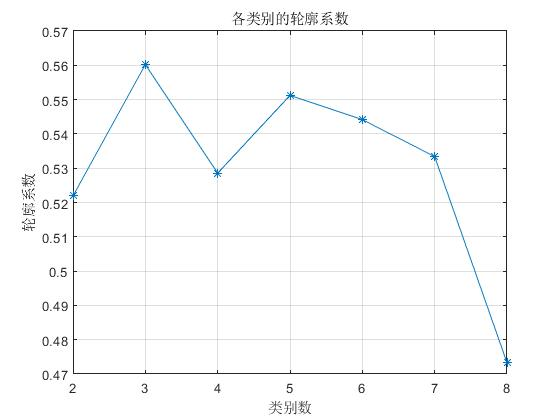
\includegraphics[width=13cm]{figure/lkxs.jpg}
    \caption{轮廓系数}
    \label{fig:lkxs}
\end{figure}
则最优的分类数为3,然后运行子程序,得到如下结果:
\begin{figure}[H]
    \centering
    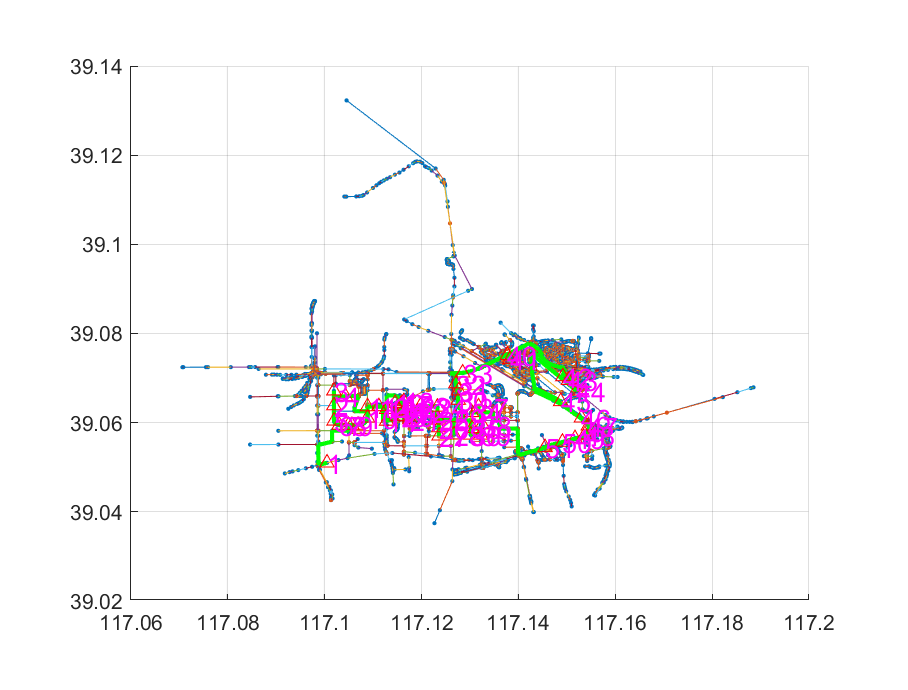
\includegraphics[width=13cm]{figure/city_path.eps}
    \caption{运输路线图}
    \label{fig:city_path}
\end{figure}
上面为城市路线图,正三角形标记了每一个需要送达的每一个地点,路径通过绿色路线来标注,由于地图点集过多,点集距离跨度较大,导致无法较为清晰的看到其运输路径,所以我们简化了了的路径图像如下:
\begin{figure}[H]
    \centering
    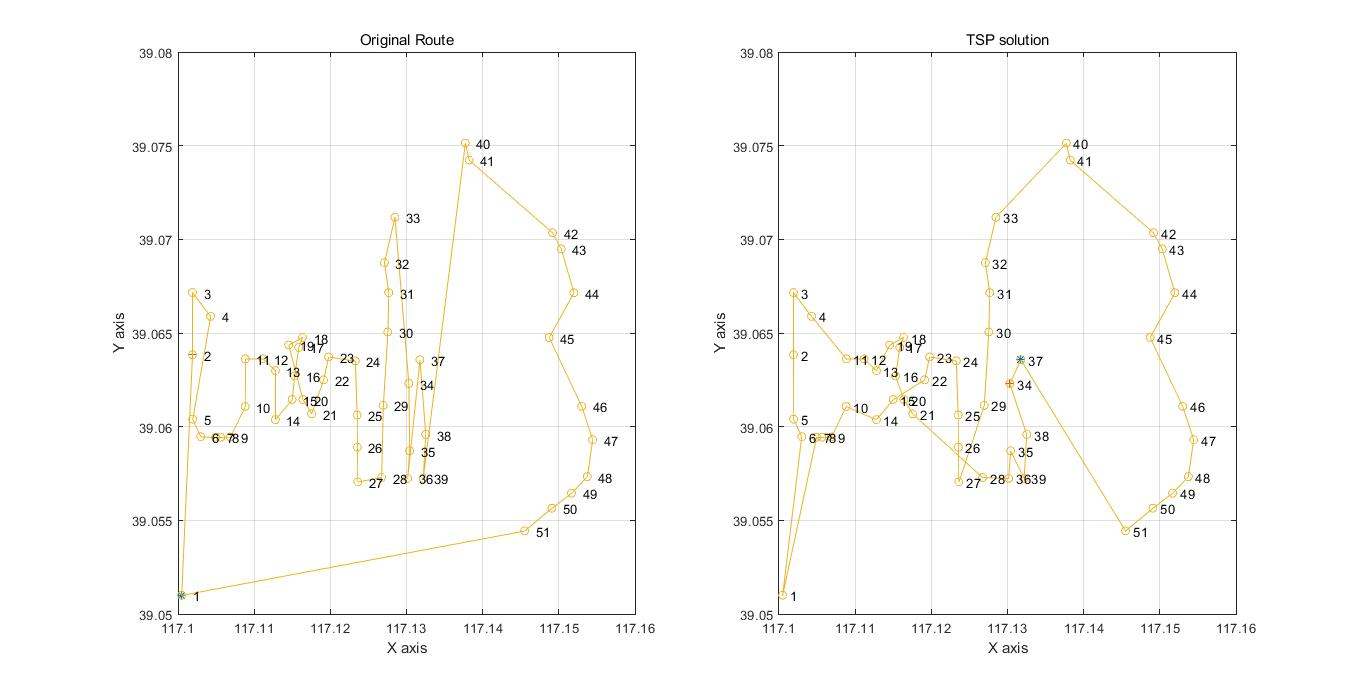
\includegraphics[width=13cm]{figure/easy_path.jpg}
    \caption{简化运输路线}
    \label{fig:easy_path}
\end{figure}
上图为简化版的运输路线,从上面我们可以看出经过程序优化过的路线图相较于人工绘制的路线图路径更加简单,在配送时间上更加快速程序中hopfield的能量函数如下:
\begin{figure}[H]
    \centering
    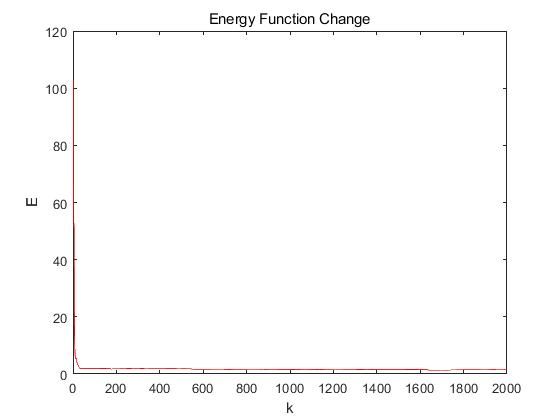
\includegraphics[width=13cm]{figure/E_diedai.jpg}
    \caption{能量函数}
    \label{fig:E_diedai}
\end{figure}
此外为了对比此算法的优越性,将GASA-hopfield算法与常见的用于解决TSP问题的智能算法效率进行比较,结果如下:
\begin{figure}[H]
    \centering
    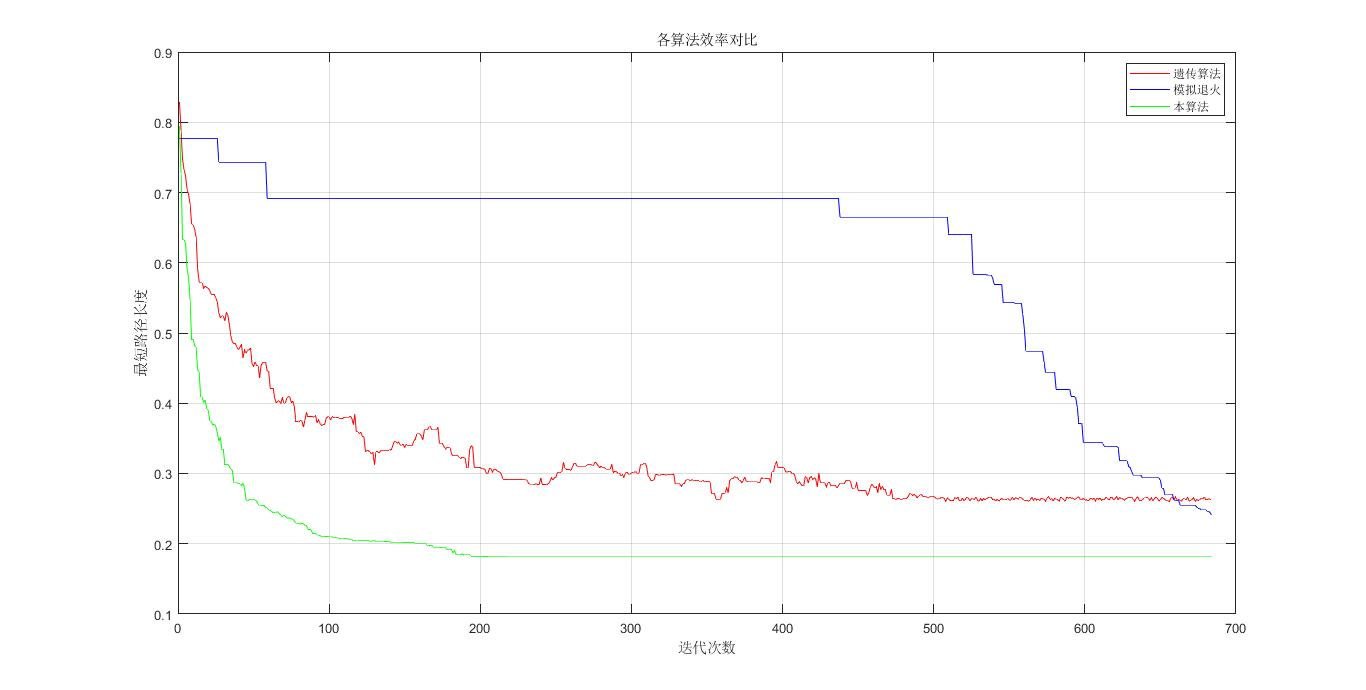
\includegraphics[width=13cm]{figure/diedai_1.jpg}
    \caption{各算法效率对比图}
    \label{fig:diedai_1}
\end{figure}
可以看出GASA-Hopfield混合优化算法的收敛的比模拟退火与遗传更快,并且也更早的找到了最优解,有趣的是遗传算法由于参数设置的较差所以导致其陷入了局部最优解,而模拟退火算法则到了700此迭代也没有彻底收敛,由此可见本算法的优越性。下面我们将比较的范围扩大到常见的解决TSP问题的算法,其对比维度为,求得的最优解,求得的平均解,与求解时间三个维度,运行程序,最后得到如下表格:
% Table generated by Excel2LaTeX from sheet 'Sheet1'
\begin{table}[H]
    \centering
    \caption{各算法运行效率}
      \begin{tabular}{|l|r|r|l|}
        \hline 
      算法    & \multicolumn{1}{l|}{最优解} & \multicolumn{1}{l|}{平均解} & 运行时间 \\
      \hline 
      暴力穷举  & 0.18121 & 0.18121 & 1000s+ \\

      剪枝    & 0.18121 & 0.18121 & 1000s+ \\

      粒子群   & 0.25  & 0.27  & 119s \\

      模拟退火  & 0.23  & 0.25  & 30s \\

      遗传    & 0.27  & 0.28  & 729s \\

      蚁群    & 0.1871 & 0.23  & 76s \\

      动态规划  & 0.18121 & 0.18121 & 1000s+ \\

      GASA-Hopfield & 0.18121 & 0.218 & 53s \\
      \hline 
      \end{tabular}%
    \label{tab:gsfyxxl}%各算法运行效率
  \end{table}%
  我们可以看出本算法在最优解上达到了已知的最优解0.18121,平均解的质量也是各智能算法中最优的,并且在求解时间上仅次于模拟退火算法,但仍然在可接受范围内,并且时间上也超过了蚁群遗传以及确定性算法,足以看出GASA-Hopfield算法的优越性。